\documentclass[a4paper,10pt]{article}

% import en preámbulo
\usepackage[spanish]{babel} % Idioma
\usepackage[utf8]{inputenc} % Codificación
\usepackage{comment} % Permite utilizar el entorno comment
\usepackage{amsmath}
\usepackage{amsthm}
\pagestyle {plain} % Configuración de página
\usepackage{graphicx} % Gráficos
\usepackage{titling}
\usepackage{amsfonts}
%\usepackage{subfigure}
\newcommand{\subtitle}[1]{%
  \posttitle{%
    \par\end{center}
    \begin{center}\large#1\end{center}
    \vskip0.4em}%
}
\usepackage{mathrsfs}
\usepackage[T1]{fontenc}
\usepackage[htt]{hyphenat}
\usepackage{float}
\usepackage{subcaption}
\usepackage[a4paper,top=2cm,bottom=3cm,left=2.5cm,right=2.5cm,marginparwidth=1.75cm]{geometry}
\usepackage{multirow}
\usepackage{siunitx} % For \num and \SI
\sisetup{output-exponent-marker=\ensuremath{\mathrm{e}}}
\usepackage{blindtext}
\usepackage{scrextend}
\usepackage[table]{xcolor}
\usepackage{pdfpages} % Para incluir PDF
%\addtokomafont{labelinglabel}{\sffamily} % For labeling lists
\renewcommand{\labelitemi}{$\bullet$}

\usepackage{hyperref} % Index con hipervinculos :)
\hypersetup{colorlinks,citecolor=black,filecolor=black,linkcolor=black,urlcolor=black}
%\captionsetup[figure]{labelfont={bf},name={Figura},labelsep=period}
%\captionsetup[table]{labelfont={bf},name={Tabla},labelsep=period}
\renewcommand{\spanishtablename}{Tabla}

\usepackage{etoolbox}
\makeatletter
\patchcmd{\@makecaption}
  {\scshape}
  {}
  {}
  {}
\makeatother


\usepackage{cancel}

\usepackage{empheq}

%\usepackage{minipage}

\newtheorem{mydef}{Definición}

%Directorio de imágenes
\graphicspath{{./img/}}

%Para bibliografía
\usepackage[backend=bibtex,style=numeric,sorting=none]{biblatex}
\addbibresource{bib_file.bib}

\usepackage{csquotes}

\DeclareRobustCommand*{\ora}{\overrightarrow}

% Comienzo del documento
\begin{document}

\newcommand{\HRule}{\rule{\linewidth}{0.5mm}}
\begin{center}
{\LARGE Tesis de Ingeniería Electrónica}\\[0.5cm]
\textbf{\Large Diseño y Construcción de una Computadora de Vuelo para Vehículos Autónomos con Tolerancia a Fallas}\\[0.6cm]
\end{center}

\begin{center}
        \begin{tabular}{lllll}
                Alumno: & & & & \\
                        & 98211 & Nuñez Frau Federico Ignacio & fnunezf@fi.uba.ar & %1130888185
                        \\
                & & & & \\
                Director: & & & & \\
                & 203004 & Pose Claudio & cldpose@fi.uba.ar & %1166889316
                \\ 
                & & & & \\
                Co-director: & & & & \\
                & %{\color{red} COMPLETAR} 
                & Garberoglio Leonardo & lgarberoglio@frsn.utn.edu.ar & %{\color{red} COMPLETAR}
                \\ 
        \end{tabular}
\end{center}

\vspace{0.3cm}

\begin{center}
        %{\color{red} COMPLETAR LA FECHA}
        25 de septiembre de 2023
\end{center}

\vspace{1.0cm}

\section{Descripción del Proyecto}

%El presente trabajo se enmarca en un proyecto más amplio, dirigido por el Laboratorio de Automática y Robótica de la FIUBA (LAR), el cual consiste en el desarrollo de un vehículo hexarotor tolerante a fallas. Esto contempla el diseño mecánico del vehículo, el diseño de la computadora de vuelo y su correspondiente software, el diseño e implementación de los algoritmos de control adecuados, el diseño de un sistema de estimación y control de velocidad, el diseño de algoritmos de evasión de obstáculos y el diseño de técnicas de detección e identificación de fallas en pleno vuelo.\\

%En el marco de este proyecto, el presente trabajo de Tesis tiene por objetivo el diseño y construcción de la computadora de vuelo de bajo nivel. Esto contempla el diseño de la plataforma de hardware PCB según los requerimientos del proyecto en el que se enmarca, y el diseño e implementación de la técnica utilizada para la tolerancia a fallas a partir del uso de redundancias de hardware.

%En los últimos años se ha incrementado mucho la presencia de vehículos aéreos no tripulados en espacio aéreo civil. 


En los últimos años ha habido un incremento en el uso de vehículos aéreos no tripulados para aplicaciones fuera del ámbito militar, como por ejemplo búsqueda y rescate, uso en construcciones e inspección, agricultura de precisión, vigilancia, entre otros \cite{8682048}. Teniendo en cuenta la importancia que han tomado en distintas actividades, además del hecho de que en muchas de estas aplicaciones estos sobrevuelan zonas donde circulan personas, resulta mandatorio garantizar cierto grado de confiabilidad en su funcionamiento. En vehículos aéreos tripulados como aviones comerciales y militares, es común que para ello se utilicen técnicas de tolerancia a fallas a partir de redundancias. Esto mismo ocurre con vehículos aéreos no tripulados de uso militar, aunque no es tan común en aquellos de uso civil y comercial.\\

En este contexto, el objetivo de este trabajo de Tesis es el diseño y construcción de una computadora de vuelo, con la capacidad de implementar mecanismos de tolerancia a fallas, a partir de redundancias, utilizando componentes \textit{commercial off-the-shelf} (COTS) \cite[p.~26]{EASAcots}.

\section{Antecedentes}

El Laboratorio de Automática y Robótica de la FIUBA (LAR) cuenta consigo con plataformas de computadoras de vuelo desarrolladas en el mismo laboratorio, que se utilizan con distintos fines de investigación. Estas computadoras de vuelo han ido incorporando distintas mejoras a lo largo de los años, y se han ido actualizando con nuevos componentes como sensores o microcontroladores. La primera de las versiones cuenta con un microcontrolador ARM Cortex M3, mientras que la última de estas cuenta un ARM Cortex M7 y sensores con mejor rendimiento \cite{garberoglio2019diseno}.\\


El LAR plantea diseñar un vehículo multi-rotor de seis rotores, con capacidad de tolerancia a fallas que puedan ocurrir en sensores redundantes. En este contexto, en el presente trabajo se quiere diseñar una computadora de vuelo que incorpore sensores de orientación y posición redundantes, con el objetivo de implementar técnicas de tolerancia a fallas a partir de redundancias de hardware.



%Los sistemas tolerantes a fallas aceptan que estas puedan ocurrir, pero implementan mecanismos que permiten continuar con su normal funcionamiento. La principal técnica de tolerancia a fallas es el uso de redundancias \cite{lala1994architectural}. Esto quiere decir que se replica el hardware en el sistema y cada réplica realiza la misma tarea en paralelo. Típicamente, existe una comparación entre los resultados calculados por cada una de las réplicas, con el objetivo de detectar y enmascarar las fallas. El hecho de duplicar o hasta triplicar el hardware trae consigo un incremento en el costo del vehículo. Debido a esto, se buscaron trabajos similares que preferentemente utilicen componentes COTS. Dos de los trabajos que se tendrán en cuenta para el desarrollo de esta Tesis son \cite{hiergeist2018implementation} y \cite{zhang2020architecture}. Ambos implementan mecanismos de tolerancia a fallas, utilizando componentes COTS, a través del intercambio de información entre los nodos redundantes, buscando llegar a un consenso respecto a algún dato, como puede ser una medición de un sensor. {\color{red} agregar que esto es común en aviones. Citar algo}.\\



%En \cite{hiergeist2018implementation} se implementa una arquitectura con redundancia cuádruple para un UAV. Cada uno de estos nodos se comunica con los demás a través de un periférico SPI. En \cite{zhang2020architecture}, el esquema de redundancias comprende nodos que realizan distintas tareas, lo que vuelve más complejo al sistema. Además, este utiliza un bus de comunicación, común a todos los nodos.

%En \cite{hiergeist2018implementation} se implementa una arquitectura con redundancia cuádruple para un UAV. Estos típicamente realizan las tareas de relevamiento de datos de sensores, cálculo de la ley de control y aplicación de resultados a sus actuadores, de manera periódica. La tolerancia a fallas se implementa a través del intercambio de información entre los 4 nodos, buscando lograr un consenso. Esto quiere decir que todos los nodos deben coincidir por ejemplo, en el valor de la medición de un sensor o en el resultado de un cálculo de la ley de control\\

%En \cite{zhang2020architecture}, el trabajo también implementa la tolerancia a fallas a través del intercambio de sus nodos. Este tiene la particularidad de hacer énfasis en una arquitectura gobernada por el tiempo, es decir que el vehículo funciona de una forma predefinida, lo que le da mayor determinismo y seguridad al sistema.

\section{Área/s Profesional/es de Relevancia}

Para el presente trabajo de Tesis, las áreas profesionales de relevancia encuadradas dentro del alcance del título de Ingeniero/a Electrónico/a de la UBA son las de Sistemas Digitales y Computación y Automatización y Control.

\section{Objetivo General y Objetivos Particualres}

El presente trabajo de Tesis tiene por objetivo el diseño y construcción de una computadora de vuelo de bajo nivel, a ser utilizada en un vehíuclo aéreo hexarotor, no tripulado. Como aspecto particular, esta debe contar con la capacidad de tolerar ciertas fallas de hardware que puedan ocurrir en pleno vuelo. Lo que se busca, es que estas fallas no impacten en la misión del vehículo y que puedan ser detectadas lo antes posible para tomar una acción.\\

El presente trabajo se enmarca en un proyecto más amplio, dirigido por el Laboratorio de Automática y Robótica de la FIUBA (LAR), el cual consiste en el desarrollo de un vehículo hexarotor tolerante a fallas. Esto contempla el diseño mecánico del vehículo, el diseño de la computadora de vuelo y su correspondiente software, el diseño e implementación de los algoritmos de control adecuados, el diseño de un sistema de estimación y control de velocidad, el diseño de algoritmos de evasión de obstáculos y el diseño de técnicas de detección e identificación de fallas en pleno vuelo.

Los objetivos particulares son:

\begin{itemize}
    \item Entender el estado del arte, en cuanto a tolerancia de fallas en vehículos aéreos no tripulados.
    \item Diseño y construcción de la computadora de vuelo.
    \item Pruebas del correcto funcionamiento de la misma.
    \item Desarrollo de un prototipo que ejecute un mecanismo de tolerancia a fallas.
    \item Validación del prototipo, simulando distintos tipos de fallas en el vehículo.
\end{itemize}

\section{Definición de la Necesidad y Evaluación Preliminar de las Soluciones Existentes}



%Los sistemas tolerantes a fallas aceptan que estas puedan ocurrir, pero implementan mecanismos que permiten continuar con su normal funcionamiento. La principal técnica de tolerancia a fallas es el uso de redundancias \cite{lala1994architectural}. Esto quiere decir que se replica el hardware en el sistema y cada réplica realiza la misma tarea en paralelo. Típicamente, existe una comparación entre los resultados calculados por cada una de las réplicas, con el objetivo de detectar y enmascarar las fallas. El hecho de duplicar o hasta triplicar el hardware trae consigo un incremento en el costo del vehículo.\\

Se buscaron trabajos similares que preferentemente utilicen componentes COTS. Dos de los trabajos que se tendrán en cuenta para el desarrollo de esta Tesis son \cite{hiergeist2018implementation} y \cite{zhang2020architecture}. Ambos implementan mecanismos de tolerancia a fallas, utilizando componentes COTS, a través del intercambio de información entre los nodos redundantes, buscando llegar a un consenso respecto a algún dato, como puede ser una medición de un sensor. {\color{red} agregar que esto es común en aviones. Citar algo}. En \cite{hiergeist2018implementation} se implementa una arquitectura con redundancia cuádruple para un UAV. Estos típicamente realizan las tareas de relevamiento de datos de sensores, cálculo de la ley de control y aplicación de resultados a sus actuadores, de manera periódica. La tolerancia a fallas se implementa a través del intercambio de información entre los 4 nodos, buscando lograr un consenso. Esto quiere decir que todos los nodos deben coincidir por ejemplo, en el valor de la medición de un sensor o en el resultado de un cálculo de la ley de control. Por otro lado, en \cite{zhang2020architecture}, el trabajo también implementa la tolerancia a fallas a través del intercambio de sus nodos. Este tiene la particularidad de hacer énfasis en una arquitectura gobernada por el tiempo, es decir que el vehículo funciona de una forma predefinida, lo que le da mayor determinismo y seguridad al sistema. Esto se traduce en que los nodos trabajan de manera sincronizada.\\

El desarrollo del presente trabajo tendrá en cuenta los requerimientos típicos de un sistema tolerante a fallas, de tiempo real. Se tendrán en cuenta los requerimientos del laboratorio en cuanto a los sensores e interfaces de comunicación necesarias, en particular en la interfaz de comunicación necesaria para implementar el mecanismo de tolerancia a fallas.

\section{Descripción del Alcance del Proyecto y Planteo de los Mecanismos que se Utilizarán para Verificar la Calidad de los Resultados Obtenidos}

La principal tarea consiste en el diseño y el desarrollo de la computadora de vuelo, teniendo en cuenta los requerimientos planteados por el proyecto en el que se enmarca. Para ello se realizarán las siguientes tareas:

\begin{itemize}
    \item Recolectar información sobre las normas comerciales para el hardware, respecto a requerimientos de cada uno de los posibles integrados, componentes, y diseño de un PCB. %Observar requerimientos para conectores, redundancia, normas de sellado, etc.
    \item Selección de componentes físicos para una computadora de vuelo. Esto comprende los distintos tipos de sensores necesarios, los módulos que debe controlar la computadora de vuelo y las interfaces de comunicación externas. Particularmente, se tendrá en cuenta la necesidad del stacking de múltiples controladoras de vuelo para redundancia.
    \item Diseño del circuito esquemático y desarrollo de la placa de circuito impreso de la computadora de vuelo, teniendo en cuenta aspectos de manufacturabilidad.
    \item Análisis de los requerimientos y las características de un sistema tolerante a fallas de tiempo real.
    \item Construcción de un prototipo que demuestre la capacidad de tolerar fallas, en la computadora de vuelo. 
\end{itemize}


\section{Definición de los Entregables}

Se presenta una lista de los entregables. A su vez, en la figura \ref{fig:cronograma_actividades}, se adjunta un cronograma de actividades.

\begin{itemize}
    \item Circuito esquemático y diseño de la placa de circuito impreso de la computadora de vuelo, junto con la correspondiente lista de componentes.
    \item Computadora de vuelo funcional, con la correspondiente interfaz de comunicación para implementar algoritmos de tolerancia a fallas.
    \item Evidencias que demuestren la capacidad de tolerancia a fallas de la computadora de vuelo, a partir de la construcción de un prototipo funcional.
    \item Informe final del trabajo.
\end{itemize}

\begin{figure}[H]
    \centering
    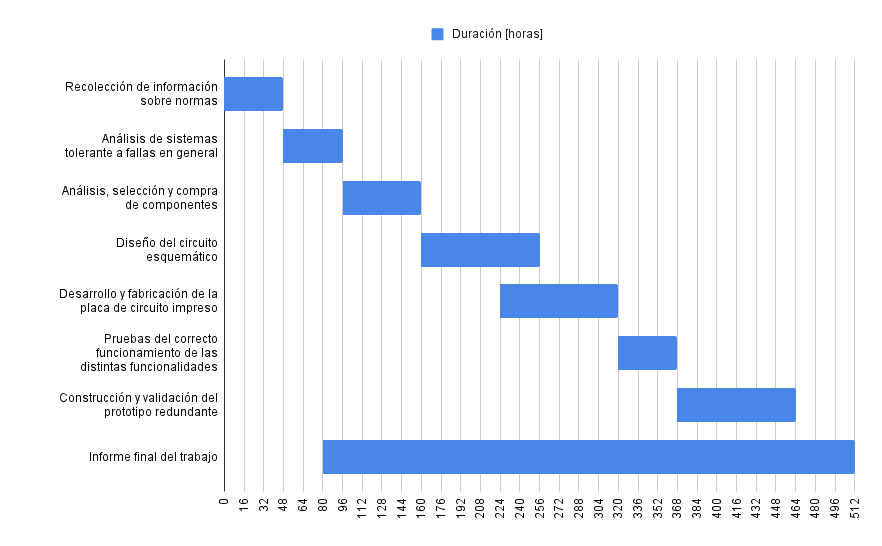
\includegraphics[width=0.9\textwidth]{img/plan_de_actividades_tentativo.png}
    \caption{Cronograma de actividades.}
    \label{fig:cronograma_actividades}   
\end{figure}

\printbibliography[heading=bibintoc]

\end{document}
